\chapter{Results}
\section{\label{section:the_data}The AOLME Dataset}
The AOLME dataset is an enormous repository of over 900 hours of video
recordings of students. The videos contain students
interacting with facilitators, their peers and computers to write code in
Python on the Raspberry Pi.  The dataset is wealth of information but difficult
to exploit in its current state.  The data used for this thesis is a subset of
the entire AOLME dataset. By hand, we have selected several videos and extracted
typing and writing clips from the original dataset and are using these as ground
truth for measuring the accuracy of our methods. Figure \ref{fig:typing_writing}
is representative of the features that have been extracted by hand.

\begin{figure}[h]
  \label{fig:typing_writing}
  \centering
  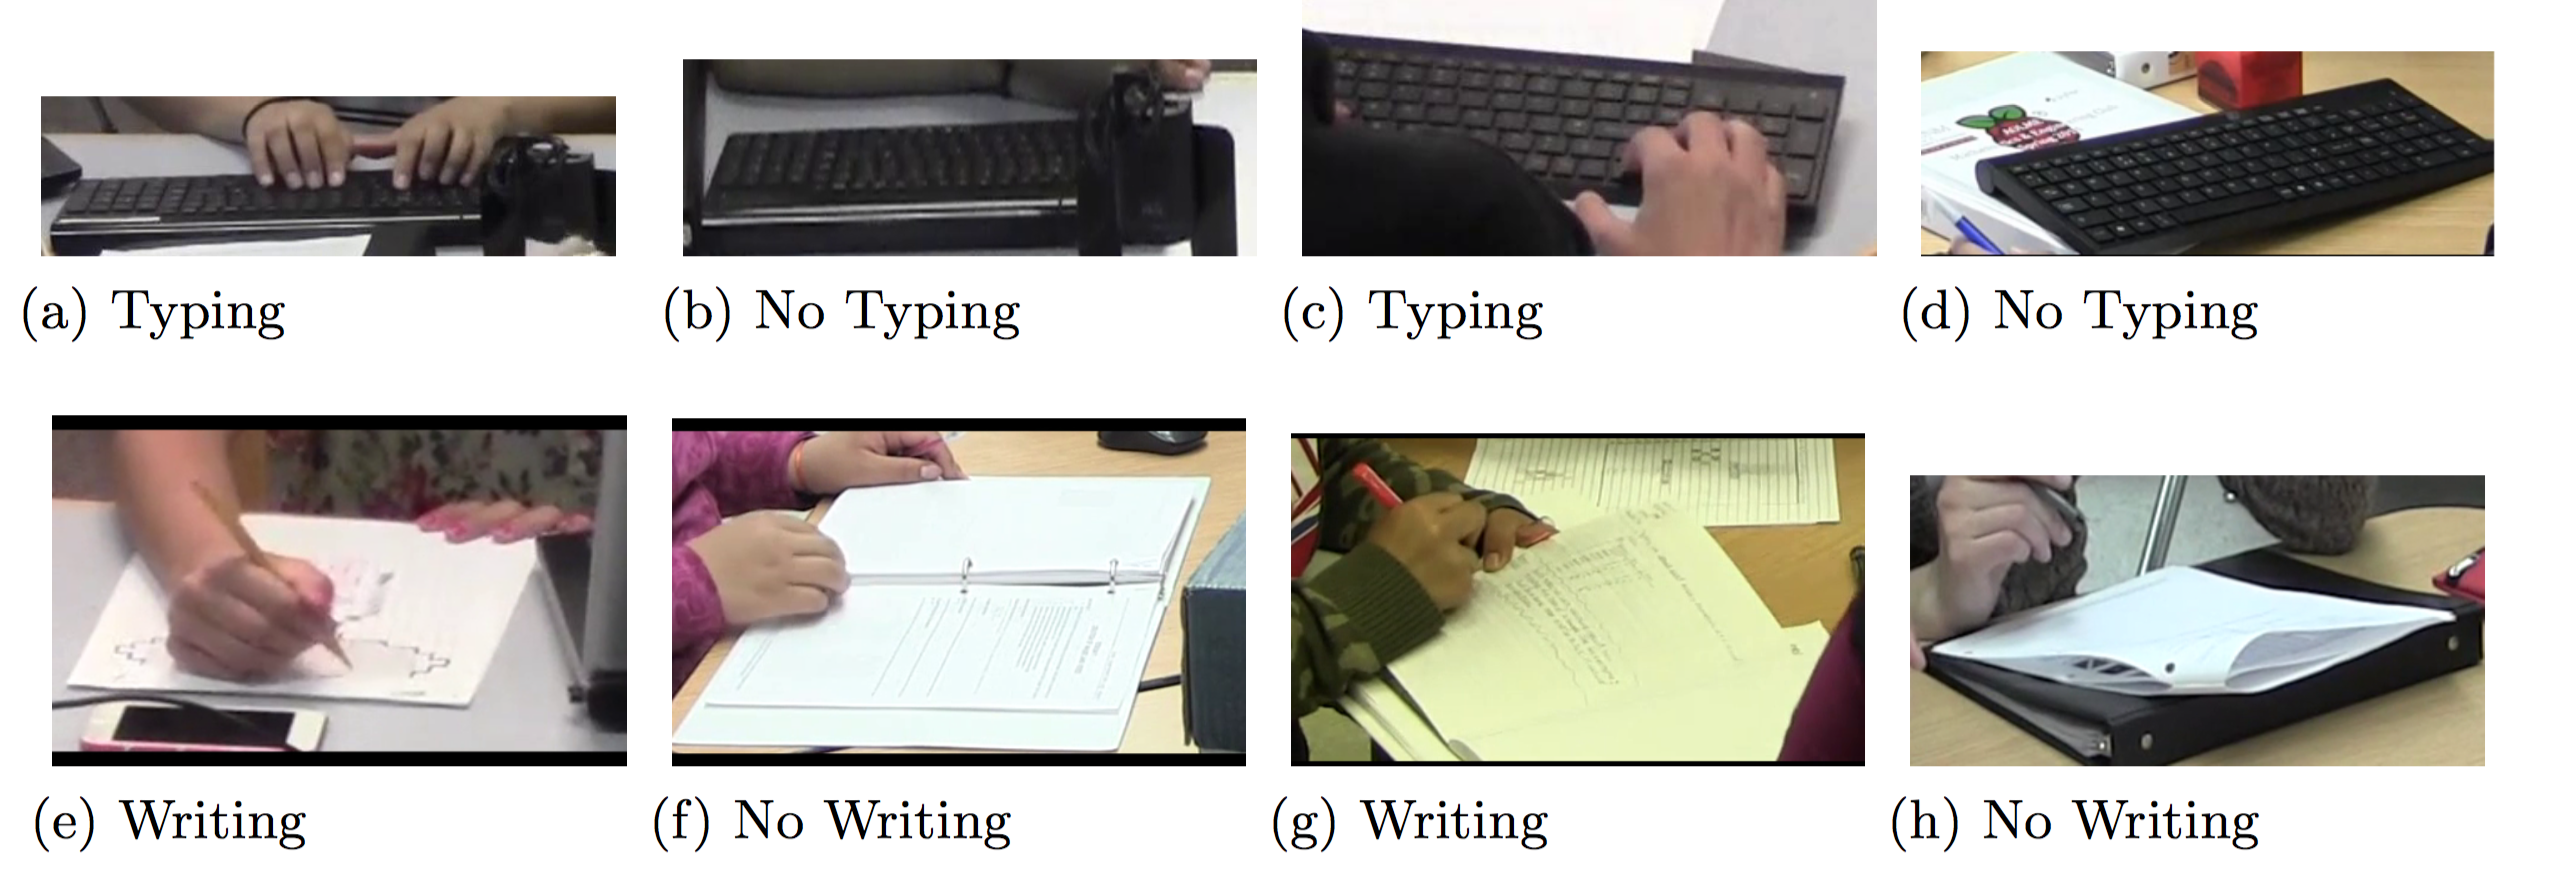
\includegraphics[width=\textwidth]{figures/typing_writing_clip}
  \caption{Example of features that have been manually extracted from the dataset
  for training and testing. For the above example, we need to classifiers for each
  activity to determine if the activity is being performed, or it is not.}
\end{figure}

As Figure \ref{fig:typing_writing} suggests, we are only using a cropped version
of the video. The reason for this is that we are not attempting to solve the tracking
problem in this thesis, only the classification problem. Hence, we assume that
the videos entering into our software have already been clipped and cropped with
the target activities inside of them and the corresponding lack of the activity.
Our subset of the AOLME database consists of the following:

\begin{itemize}
\item Twenty videos of typing
\item Twenty videos of no typing
\item Twenty videos of writing
\item Twenty Videos of no writing
\end{itemize}

\section{\label{section:accuracy} Accuracy of Classification}
In this section we explore how well our results are for both the classification
of typing and writing videos using the techniques described in methods chapter.

For our first set of results, we ran to classifying typing motions in videos.
The input messages into the cluster are shown in Table \ref{table:typing_messages}.
The original dataset, however, contains 10-20 for each of the training classifications,
we have left them out in this table for brevity.
\begin{table}[h]
  \label{table:message_queue}
  \begin{tabular}{ | l | l | l | p{3cm} |}
  \hline
  \textbf{path} & \textbf{classification} & \textbf{sqs\_queue} & \textbf{of\_algorithm}\\ \hline
  aolme/data/typing/seg\_1.mp4 & 1 & feature\_queue & farneback\\\hline
  aolme/data/typing/seg\_2.mp4 & 1 & feature\_queue & farneback\\\hline
  aolme/data/typing/seg\_3.mp4 & 1 & feature\_queue & farneback\\\hline
  aolme/data/typing/seg\_4.mp4 & 1 & feature\_queue & farneback\\\hline
  aolme/data/typing/seg\_5.mp4 & 1 & feature\_queue & farneback\\\hline
  aolme/data/typing/seg\_6.mp4 & 1 & feature\_queue & farneback\\\hline
  aolme/data/typing/seg\_7.mp4 & 1 & feature\_queue & farneback\\\hline
  aolme/data/typing/seg\_8.mp4 & 1 & feature\_queue & farneback\\\hline
  aolme/data/typing/seg\_9.mp4 & 1 & feature\_queue & farneback\\\hline
  aolme/data/typing/seg\_10.mp4 & 1 & feature\_queue & farneback\\\hline
  aolme/data/notyping/seg\_1.mp4 & 2 & feature\_queue & farneback\\\hline
  aolme/data/notyping/seg\_2.mp4 & 2 & feature\_queue & farneback\\\hline
  aolme/data/notyping/seg\_3.mp4 & 2 & feature\_queue & farneback\\\hline
  aolme/data/notyping/seg\_4.mp4 & 2 & feature\_queue & farneback\\\hline
  aolme/data/notyping/seg\_5.mp4 & 2 & feature\_queue & farneback\\\hline
  aolme/data/notyping/seg\_6.mp4 & 2 & feature\_queue & farneback\\\hline
  aolme/data/notyping/seg\_7.mp4 & 2 & feature\_queue & farneback\\\hline
  aolme/data/notyping/seg\_8.mp4 & 2 & feature\_queue & farneback\\\hline
  aolme/data/notyping/seg\_9.mp4 & 2 & feature\_queue & farneback\\\hline
  aolme/data/notyping/seg\_10.mp4 & 2 & feature\_queue & farneback\\\hline
  \end{tabular}
  \caption{Data that is sent to the SQS for calculation on the cluster. The
  original dataset includes 10-20 for both classifications}
\end{table}

Using our R code, we then plot some statistics about the vectors that have come
back from the cluster. This is shown in figure \ref{fig:typing_box_whiskers}.
The first column represents the statistics from videos that have the activity
in them, and the second column represents the lack of that activity. Just from
visual inspection, we can already see that there differences in the overall
statistics, which means that we should have very good luck with our support
vector machine properly classifying the results.

\FloatBarrier

\begin{figure}[h]
  \label{fig:typing_box_whiskers}
  \centering
  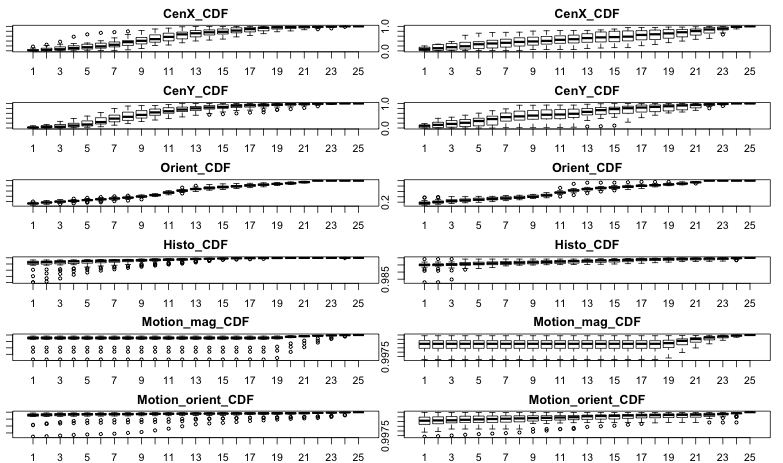
\includegraphics[width=\textwidth]{figures/typing_box_whiskers}
  \caption{Box and whiskers plot of CDFs for typing. The first column represents the
  statistics for typing and the second column represents the statistics for no
  writing.}
\end{figure}

With those feature vectors, we found that we were able to get the confusion matrix
shown in Table \ref{table:typing_confusion}
\begin{table}[h]
  \begin{centering}
  \label{table:typing_confusion}
  \begin{tabular}{| l | l | l |}
  \hline
   & \textbf{typing} & \textbf{no typing}\\ \hline
  \textbf{typing} & 19 & 1 \\ \hline
  \textbf{no typing} & 3 & 17 \\ \hline
  \end{tabular}
  \caption{Confusion matrix for classification accuracy for typing}
\end{centering}
\end{table}

\FloatBarrier

From Table \ref{table:typing_confusion} we can see that we get 90\% accuracy for
classifying typing motions on the keyboard. We had difficulty classifying
videos that had significant motion in them, but the motion was not typing and
we also found that we had trouble classifying the videos where there is was
not much typing in the videos that were classified as typing. But overall, when the
scene clearly had typing and when it clearly did not, we found that we had
90\% accuracy.

Our results for determining writing, however, were not as good as our results
for classifying typing. Our CDFs for typing are shown in figure

\begin{figure}[h]
  \label{fig:typing_box_whiskers}
  \centering
  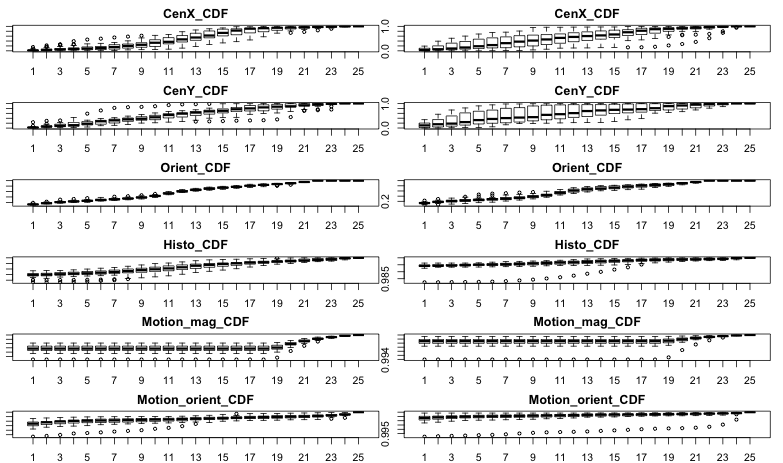
\includegraphics[width=\textwidth]{figures/writing_cdfs}
  \caption{Box and whiskers plot of CDFs for writing. The first column represents the
  statistics for typing and the second column represents the statistics for no
  writing.}
\end{figure}

\begin{table}[h]
  \begin{centering}
  \label{table:writing_confusion}
  \begin{tabular}{| l | l | l |}
  \hline
   & \textbf{writing} & \textbf{no writing}\\ \hline
  \textbf{writing} & 18 & 2 \\ \hline
  \textbf{no writing} & 11 & 9 \\ \hline
  \end{tabular}
  \caption{Confusion matrix for classification accuracy for typing}
\end{centering}
\end{table}
